\documentclass[a4paper,11pt]{article}
\usepackage[utf8]{inputenc}
\usepackage[russian]{babel}
\usepackage[T1]{fontenc}
\usepackage{amssymb,amsmath,graphicx,indentfirst}
\usepackage{caption}
\usepackage{clrscode}
\usepackage[unicode]{hyperref}

\setlength{\parskip}{1ex plus 0.5ex minus 0.2ex}
\newcommand\doubleplus{+\kern-1.3ex+\kern0.8ex}

\author{Олег Смирнов\\
\texttt{oleg.smirnov@gmail.com}}
\date{24 ноября 2011 г.}
\title{Построение и анализ алгоритмов -- Лекция 8. Динамическое
программирование, часть 1}

\begin{document}

\maketitle
\tableofcontents
\newpage

\setlength{\parskip}{1ex plus 0.5ex minus 0.2ex}

\section*{Цель лекции}
\begin{itemize}
\item Понятие динамического программирования
\item Задача поиска наибольшей общей подстроки
\item Редакторское расстояние
\item Задача о перемножении цепочки матриц
\item Задача о пути в графе
\item Задача о наибольшей возрастающей подпоследовательности
\end{itemize}

\section{Введение}
Слово ``программирование'' в названии метода не относится к программированию как
к написанию программ, так же как и в ``линейном программировании''. Исторически
так называли табличные методы, как в случае перфокарт.

Динамическое программирование является методом дизайна алгоритмов, наряду с такими
методами как ``разделяй и властвуй'', ``жадные алгоритмы'', ``рандомизация'' и т.д.

\section{Задача поиска наибольшей общей подстроки}
Хорошим примером применения метода является задача поиска наибольшей общей
подпоследовательности (англ. Longest Common Subsequence, LCS).

Для двух заданных строк (множеств элементов) $x[1 \twodots m]$ и $y[1 \twodots n]$
найти наибольшие общие последовательности элементов (их может быть несколько).

Задача возникает, например, в вычислительной биологии, где требуется сравнивать
цепочки ДНК.

В этом примере $LCS(x, y) = BCBA, BDAB, BCAB, \twodots$.
\begin{center}
\begin{tabular}{|r|c|c|c|c|c|c|c|}
  \hline
     $x$ & A & B & C & B & D & A & B \\
  \hline
     $y$ & B & D & C & A & B & A &   \\
  \hline
\end{tabular}
\end{center}

В случае наивного алгоритма поиска $LCS$: для каждой подпоследовательности из
$x$ проверить, содержится ли она в $y$. Тогда:
\begin{itemize}
\item время проверки каждой подпоследовательности в $y$: $O(n)$;
\item общее количество подпоследовательностей в $x$: $2^m$ (рассматриваем вектор
битов длиной $m$, каждый бит которого означает, включать ли соответствующий
элемент);
\item время работы алгоритма в худшем случае: $O(n \cdot 2^m)$ -- экспоненциальное.
\end{itemize}

Более оптимальный алгоритм поиска $LCS$ состоит из двух шагов:
\begin{enumerate}
\item Вычисление \emph{длины} наибольшей общей подпоследовательности
\item Поиск подпоследовательности заданной длины
\end{enumerate}

Очевидно, что наибольшая длина, полученная на первом шаге, является искомой.
Алгоритм становится проще за счёт того, что необходимо работать только с
числами -- длинами $LCS$. Обозначим длину последовательности $s$ через $|s|$.

Важным шагом в дизайне алгоритмов динамического программирования является
рассмотрение подзадач. Необходимо показать, что оптимальное решение исходной
задачи содержит оптимальные решения подзадач меньшего размера.

Рассмотрим \emph{префиксы} $x$ и $y$. 

Пусть $c[i, j] = |LCS(x[1 \twodots i], y[1 \twodots j])|$ -- длина общей
подпоследовательности для префиксов $x$ и $y$ длины $i$ и $j$
соответственно. Вычислив для всех $i$ и $j$, получим
$c[m, n] = |LCS(x, y)|$ -- искомая наибольшая подпоследовательность.

Значение $c[i, j]$ можно вычислить рекурсивно. Докажем теорему:
\begin{equation*}
  c[i, j] = \begin{cases}
    c[i-1, j-1] + 1, \text{ если } x[i] = y[j] \\
    max\{c[i-1, j], c[i, j-1]\}, \text{ в противном случае}
    \end{cases}
\end{equation*}

Т.е. длина общей последовательности двух префиксов на единицу больше
предыдущих префиксов, если их конечные элементы совпадают, или равна
максимуму из двух длин для двух предыдущих префиксов в противном случае.
\begin{figure}[ht]
  \centering
  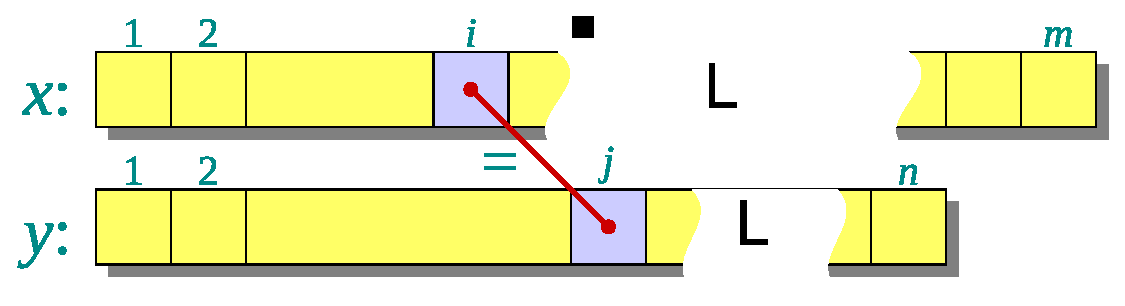
\includegraphics[width=3.5in]{lecture8/lcs.eps}
  \caption{Задача LCS}
\end{figure}

Рассмотрим случай $x[i] = y[j]$.

Пусть $z[1 \twodots k] = LCS(x[1 \twodots i], y[1 \twodots j])$ -- $LCS$
префиксов, тогда $c[i, j] = k$ -- длина $z$. Тогда последний символ
подпоследовательности должен быть равен $z[k] = x[i] (= y[j])$ иначе $z$
можно было бы удлинить, добавив $x[i]$.

Следствие: $z[1 \twodots k-1]$ является наибольшей подпоследовательностью
префиксов: 
\begin{equation*}
  z[1 \twodots k-1] = LCS(x[1 \twodots i-1], y[1 \twodots j-1])  
\end{equation*}

Допустим, $w$ -- общая подпоследовательность $x[1 \twodots i-1]$ и
$y[1 \twodots j-1]$, которая длиннее $z$. Т.е. $|w| > k-1$. Тогда конкатенация
$w \doubleplus z[k]$ также является общей подпоследовательностью 
$x[1 \twodots i]$, $y[1 \twodots j]$ длины $|w \doubleplus z[k]| > k$.
Но это невозможно, т.к. длина наибольшей общей подпоследовательности
исходных строк равна $k$ по условию. Это противоречие доказывает следствие.
Такой аргумент называется ``cut and paste''.

Таким образом $c[i-1, j-1] = k-1$, откуда следует, что $c[i, j] = 
c[i-1, j-1] +1$. Остальные случаи симметричны.

Это свойство называется ``оптимальной подструктурой'' или первым признаком
динамического программирования.

\emph{Первый признак динамического программирования}: оптимальное решение
исходной задачи содержит оптимальные решения подзадач меньшего размера.

В случаи задачи $LCS$ это означает, что если $z = LCS(x, y)$, то любой
префикс $z$ является $LCS$ префикса $x$ и префикса $y$.

Для проверки первого признака обычно используют аргумент ``cut and paste''.

Используя теорему, можно записать рекурсивный алгоритм:
\begin{codebox}
\Procname{$\proc{LCS}(x, y, i, j)$}
\li \If $x[i] = y[i]$
\li   \Then $c[i,j] \gets LCS(x, y, i-1, i-1)+1$
\li   \Else $c[i,j] \gets max\{LCS(x, y, i-1, j), LCS(x, y, i, j-1)\}$
    \End
\li \Return $c[i,j]$
\end{codebox}
В худшем случае, если $x[i] \neq y[j]$ алгоритм выполняет рекурсивное 
вычисление двух подзадач, по очереди декрементируя один из параметров.
\begin{figure}[h!]
  \centering
  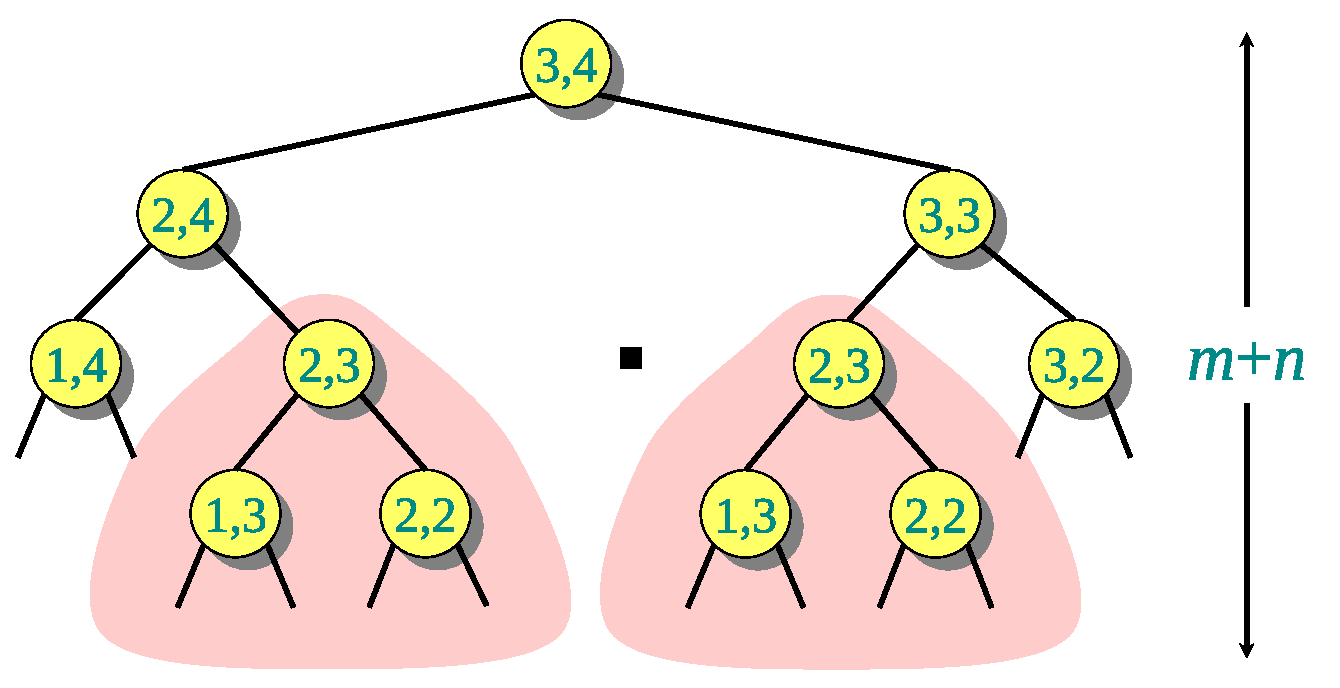
\includegraphics[width=3.5in]{lecture8/tree.eps}
  \caption{Дерево рекурсии}
\end{figure}
Дерево рекурсии алгоритма имеет высоту $m+n$, т.е. время выполнения 
попрежнему будет экспоненциальным.

Можно заметить, что некоторые поддеревья в нём повторяются несколько раз.
Вычисляя соответствующие подзадачи однократно, время работы можно сократить.

Это свойство называется ``перекрывающимися подзадачами'' или вторым признаком
динамического программирования.

\emph{Второй признак динамического программирования}: рекурсивное решение
содержит небольшое количество различных подзадач, которые повторяются многократно.

Количество различных подзадач в $LCS$ равно $n \cdot m$, что гораздо меньше
 $n \cdot 2^m$.

\section{Мемоизация}
Для решения можно применить подход, называемый мемоизацией (memoization): после
вычисления решения подзадачи оно записывается в таблицу и при повторном вызове
уже не вычисляется, а берётся из таблицы.

\begin{codebox}
\Procname{$\proc{LCS}(x, y, i, j)$}
\li \If $c[i,j] = NIL$
\li \Then \If $x[i] = y[i]$
\li     \Then $c[i,j] \gets LCS(x, y, i-1, i-1)+1$
\li     \Else $c[i,j] \gets max\{LCS(x, y, i-1, j), LCS(x, y, i, j-1)\}$
      \End
    \End
\li \Return $c[i,j]$
\end{codebox}
Амортизированное время работы этого алгоритма $T(m, n) = \Theta(m \cdot n)$.
Объем используемой памяти $Space(m, n) = \Theta(m \cdot n)$.

Мемоизация хорошо подходит для функций, которые возвращают одинаковые значения
для одинаковых входных параметров. Этот приём не работает для функций с
побочными эффектами.

\section{Динамическое программирование}
Алгоритм с мемоизацией использует значительный объём памяти и выполняет
вычисления в обратном порядке (сверху-вниз). Идея динамического программирования
заключается в том, что таблицу значений $c[i, j]$ можно вычислять
последовательно, снизу-вверх:
\begin{figure}[h!]
  \centering
  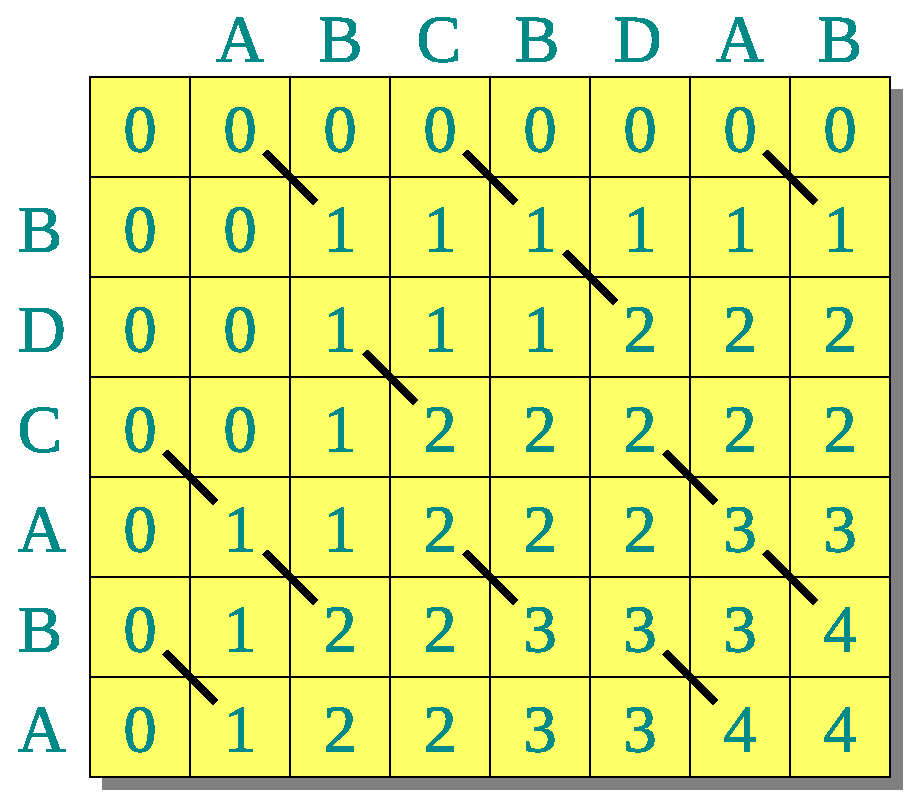
\includegraphics[width=3in]{lecture8/table1.eps}
  \caption{Таблица LCS}
\end{figure}

Порядок заполнения таблицы:
\begin{itemize}
\item первая строка и первый столбец таблицы заполняются нулями;
\item каждый элемент последовательно заполняется по формуле для $c[i, j]$: если
символы для позиции $i, j$ совпадают, то в неё записывается значение
$c[i-1, j-1]+1$, иначе вычисляется максимум от соседей слева и сверху.
\end{itemize}
Элемент в правом нижнем углу показывает длину наибольшей общей
подпоследовательности. Для построения искомой последовательности нужно пройти
по таблице в обратную сторону.

Порядок прохода по таблице:
\begin{itemize}
\item если элемент получен как максимум от двух префиксов -- перейти в позицию
  с наибольшим префиксом;
\item если элемент получен прибавлением единицы к соседу по диагонали -- перейти
в эту позицию и добавить соответствующий символ к последовательности;
\item выбирая различные эквивалентные пути можно получить все возможные
последовательности.
\end{itemize}
\begin{figure}[h!]
  \centering
  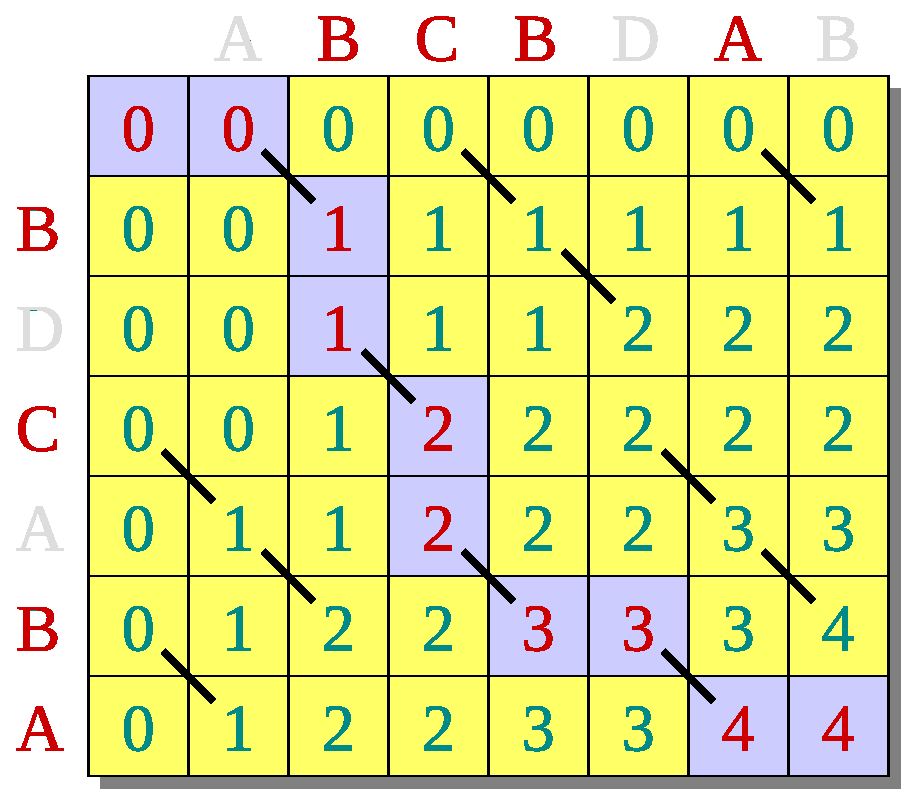
\includegraphics[width=3in]{lecture8/table2.eps}
  \caption{Таблица LCS}
\end{figure}

Алгоритм использует $\Theta(m \cdot n)$ памяти. Объем памяти можно сократить
до $O(min\{m, n\})$, если хранить вместо всей таблицы только одну (предыдущую)
строчку, которая необходима для вычисления элемента. В этом случае алгоритм
позволяет найти только \emph{длину} подпоследовательности.

Рассмотренный алгоритм LCS используется, в частности, в программе diff.
Существует еще ряд известных задач, решаемых методом динамического
программимрования.

\section{Редакторское расстояние}
Расстоянием Левенштейна (также редакторским расстоянием, editor's distance)
называется мера разницы двух последовательностей символов (строк)
относительно минимального количества операций вставки, удаления и замены,
необходимых для перевода одной строки в другую.

Задача поиска расстояния Левенштейна решается с помощью динамического
программирования. Расстояние используется в алгоритмах fuzzy matching
(например, проверка правописания) и в текстовых редакторах.

\section{Задача о перемножение цепочки матриц}
Число итераций, необходимое для умножения двух матриц размера $p \times q$
и $q \times r$ равно $p \cdot q \cdot r$. Умножение матриц ассоциативно,
т.е. три матрицы $A_1, A_2, A_3$ размерности
$10 \times 100$, $100 \times 5$ и $5 \times 50$ соответственно, можно
перемножить двумя возможными способами: $((A_1 \cdot A_2) \cdot A_3)$ и
$(A_1 \cdot (A_2 \cdot A_3))$. Однако в первом случае будет выполнено 
$10 \cdot 100 \cdot 5 + 10 \cdot 5 \cdot 50 = 7500$ итераций. А во втором
-- $100 \cdot 5 \cdot 50 + 10 \cdot 100 \cdot 50 = 75000$ итераций.

Вычислим число способов, которыми можно перемножить $n$ множителей. Оно
равно количеству вариантов расстановки скобок в выражении из $n$ членов.
Обозначим его как $P(n)$. Тогда для одного элемента $P(1) = 1$, а для 
$n \geqslant 2$ можно разбить выражение на левую часть и правую часть
между двумя любыми сомножителями. Общее количество способов тогда 
будет равно количеству сомножителей в правой части, умноженному на
количество в левой части. Запишем рекурсивную формулу:
\begin{equation*}
  P(n) = \begin{cases}
    1, \text{ если } n = 1 \\
    \sum_{k=1}^{n-1} P(k) P(n-k), \text{ если } n \geqslant 2
    \end{cases}
\end{equation*}

Можно показать, что $P(n)$ -- это число Каталана, которое оценивается как
$C_n \sim \frac{4^n}{n^{3/2}}$. Т.е. количество вариантов растёт
экспоненциально.

С помощью динамического программирования можно найти оптимальный порядок
перемножения матриц за $O(n^3)$ итераций.

Пусть $A_i A_{i+1} \ldots A_j$ -- умножение цепочки от $i$-ой до $j$-ой матрицы.
Тогда, для любого $k$, $i \leqslant k < j$ необходимо вычислить 
$A_i A_{i+1} \ldots A_k$ и $A_{k+1} \ldots A_j$, а затем перемножить результаты.

Пусть размеры матриц заданы в массиве $p$, т.е. матрица $A_i$ имеет размер
$p_{i-1} \times p_i$. Тогда элемент матрицы $m[i, j]$ -- минимальное количество
операций для вычисления произведения цепочки от $i$-ой до $j$-ой матрицы
можно вычислить рекурсивной формулой:

\begin{equation*}
  m[i, j] = \begin{cases}
    0, \text{ если } i = j \\
    \min_{i \leqslant k < j} (m[i, k] + m[k+1, j] + p_{i-1}*p_k*p_j),
    \text{ если } i < j
    \end{cases}
\end{equation*}

Последнее слагаемое во втором случае -- работа по перемножению двух матриц
размера $p_{i-1} \times p_k$ и $p_k \times p_j$.

\section{Поиск оптимального пути в графе}
Задача поиска поиска оптимальных путей из одной вершины нагруженного графа
в остальные решается алгоритмом Дейкстры (для графа без дуг отрицательного
веса) и алгоритмом Беллмана-Форда (с ними). 

При решении каждой вершине из графа $V$ сопоставляется метка -- минимальное
известное расстояние от этой вершины до начальной $a$. Алгоритм работает
пошагово -- на каждом шаге он ``посещает'' одну вершину и пытается уменьшать
метки. Работа завершается, когда все вершины посещены. В начале работы метки
вершин принимаются равными бесконечности. На каждом шаге вершины
просматриваются в порядке BFS (поиск в ширину).

Очевидно, что оптимальный путь в графе содержит подпути оптимальной длины.

Практическим приложением этого алгоритма является протокол сетевой
маршрутизации OSPF, который вычисляет оптимальный путь между узлами сети по
заданной таблице маршрутизации.

\section{Задача о наибольшей возрастающей подпоследовательности}
Пусть дан массив из $n$ чисел. Требуется найти в этой последовательности
строго возрастающую подпоследовательность наибольшей длины, т.е. 
последовательность $x[i_1] < x[i_2] < \ldots < x[i_k]$ элементов таких,
что $1 \leqslant i_1 < i_2 < \ldots < i_k < n$, причем $k$ -- наибольшее из
возможных. Эта задача известна как LIS (англ. Longest Increasing Subsequence).

Вычислим сначала длину наибольшей возрастающей подпоследовательности.

Пусть в массиве $d[0 \ldots n-1]$ элемент $d[i]$ -- это длина самой длинной
возрастающей подпоследовательности, оканчивающейся в элементе с индексом $i$.
Этот массив можно считать постепенно: сначала $d[0]$, затем $d[1]$ и т.д. В
конце, ответом к задаче будет максимальное значение в этом массиве.

Итак, пусть текущий индекс -- $i$, т.е. мы хотим посчитать значение $d[i]$, а
все предыдущие значения $d[0 \ldots i-1]$ уже подсчитаны. Возможны два варианта:
\begin{itemize}
\item либо $d[i] = 1$, т.е. искомая подпоследовательность состоит только из
  числа $a[i]$.
\item либо $d[i] > 1$. Тогда перед числом $x[i]$ в искомой подпоследовательности
  стоит какое-то другое число. Это может быть любой элемент
  $x[j], j = 0 \ldots i-1$, такой, что $x[j] < x[i]$.
\end{itemize}
Пусть мы рассматриваем какой-то текущий индекс $j$. Поскольку элемент $d[j]$ для
него уже подсчитан, то получается, что это число $a[j]$ вместе с числом $a[i]$
даёт ответ $d[j] + 1$. Таким образом, $d[j]$ можно считать по такой формуле:
\begin{equation*}
  d[i] = max_{j=0 \ldots i-1, a[j] < a[i]} (d[j] + 1)
\end{equation*}

Объединяя эти два варианта в один, получаем окончательный алгоритм для
вычисления длинны ответа:
\begin{equation*}
  d[i] = max(1, max_{j=0 \ldots i-1, a[j] < a[i]} (d[j] + 1))
\end{equation*}

Чтобы суметь восстановить ответ, помимо динамики $d$ надо также хранить
вспомогательный массив $p[0 \ldots n-1]$ с индексами значений исходной
последовательности, в которых мы достигли максимума для каждого значения
$d[i]$. Иными словами, индекс $p[i]$ будет обозначать тот самый индекс $j$, при
котором получилось наибольшее значение $d[i]$. Такой массив в динамическом
программировании часто называют ``массивом предков''.
\end{document}

